\documentclass[12pt,aspectratio=169]{beamer}

\usetheme{metropolis}

\definecolor{mDarkBrown}{HTML}{FF5722}
\definecolor{mDarkTeal}{HTML}{263238}
\definecolor{mLightBrown}{HTML}{FF5722}

\usepackage{graphicx}
\usepackage{hyphenat}
\usepackage[normalem]{ulem}

\usepackage{minted}
\usemintedstyle{tango}

\usepackage{polyglossia}
\setdefaultlanguage[variant=british]{english}
\usepackage[english=british]{csquotes}

\defaultfontfeatures{Ligatures=TeX}
\setmainfont{Lucida Sans OT}
\setsansfont[Scale=MatchLowercase]{Lucida Sans OT}
\setmonofont[Scale=MatchLowercase]{Lucida Console DK}

\author{Gianluca Campanella}
\date{}



\title{A short introduction to `--omics'}

\begin{document}

\maketitle

\begin{frame}{Contents}
    \tableofcontents
\end{frame}

\section{Molecular epidemiology}

\begin{frame}{`Hallmarks of cancer' (Hanahan and Weinberg, 2011)}
    \begin{center}
        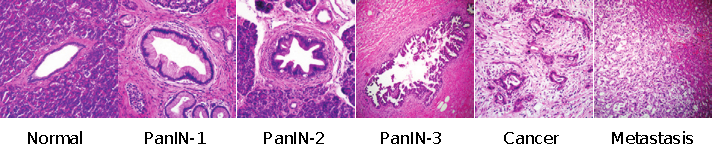
\includegraphics[width=\textwidth]{figures/pancreatic_cancer}
    \end{center}
    \vfill
    \begin{itemize}
        \item Inducing angiogenesis
        \item Resisting cell death
        \item Enabling replicative immortality
        \item Sustaining proliferative signalling
        \item Evading growth suppressors
        \item \ldots
    \end{itemize}
\end{frame}

\begin{frame}{We haven't figured it all out\ldots}
    \begin{center}
        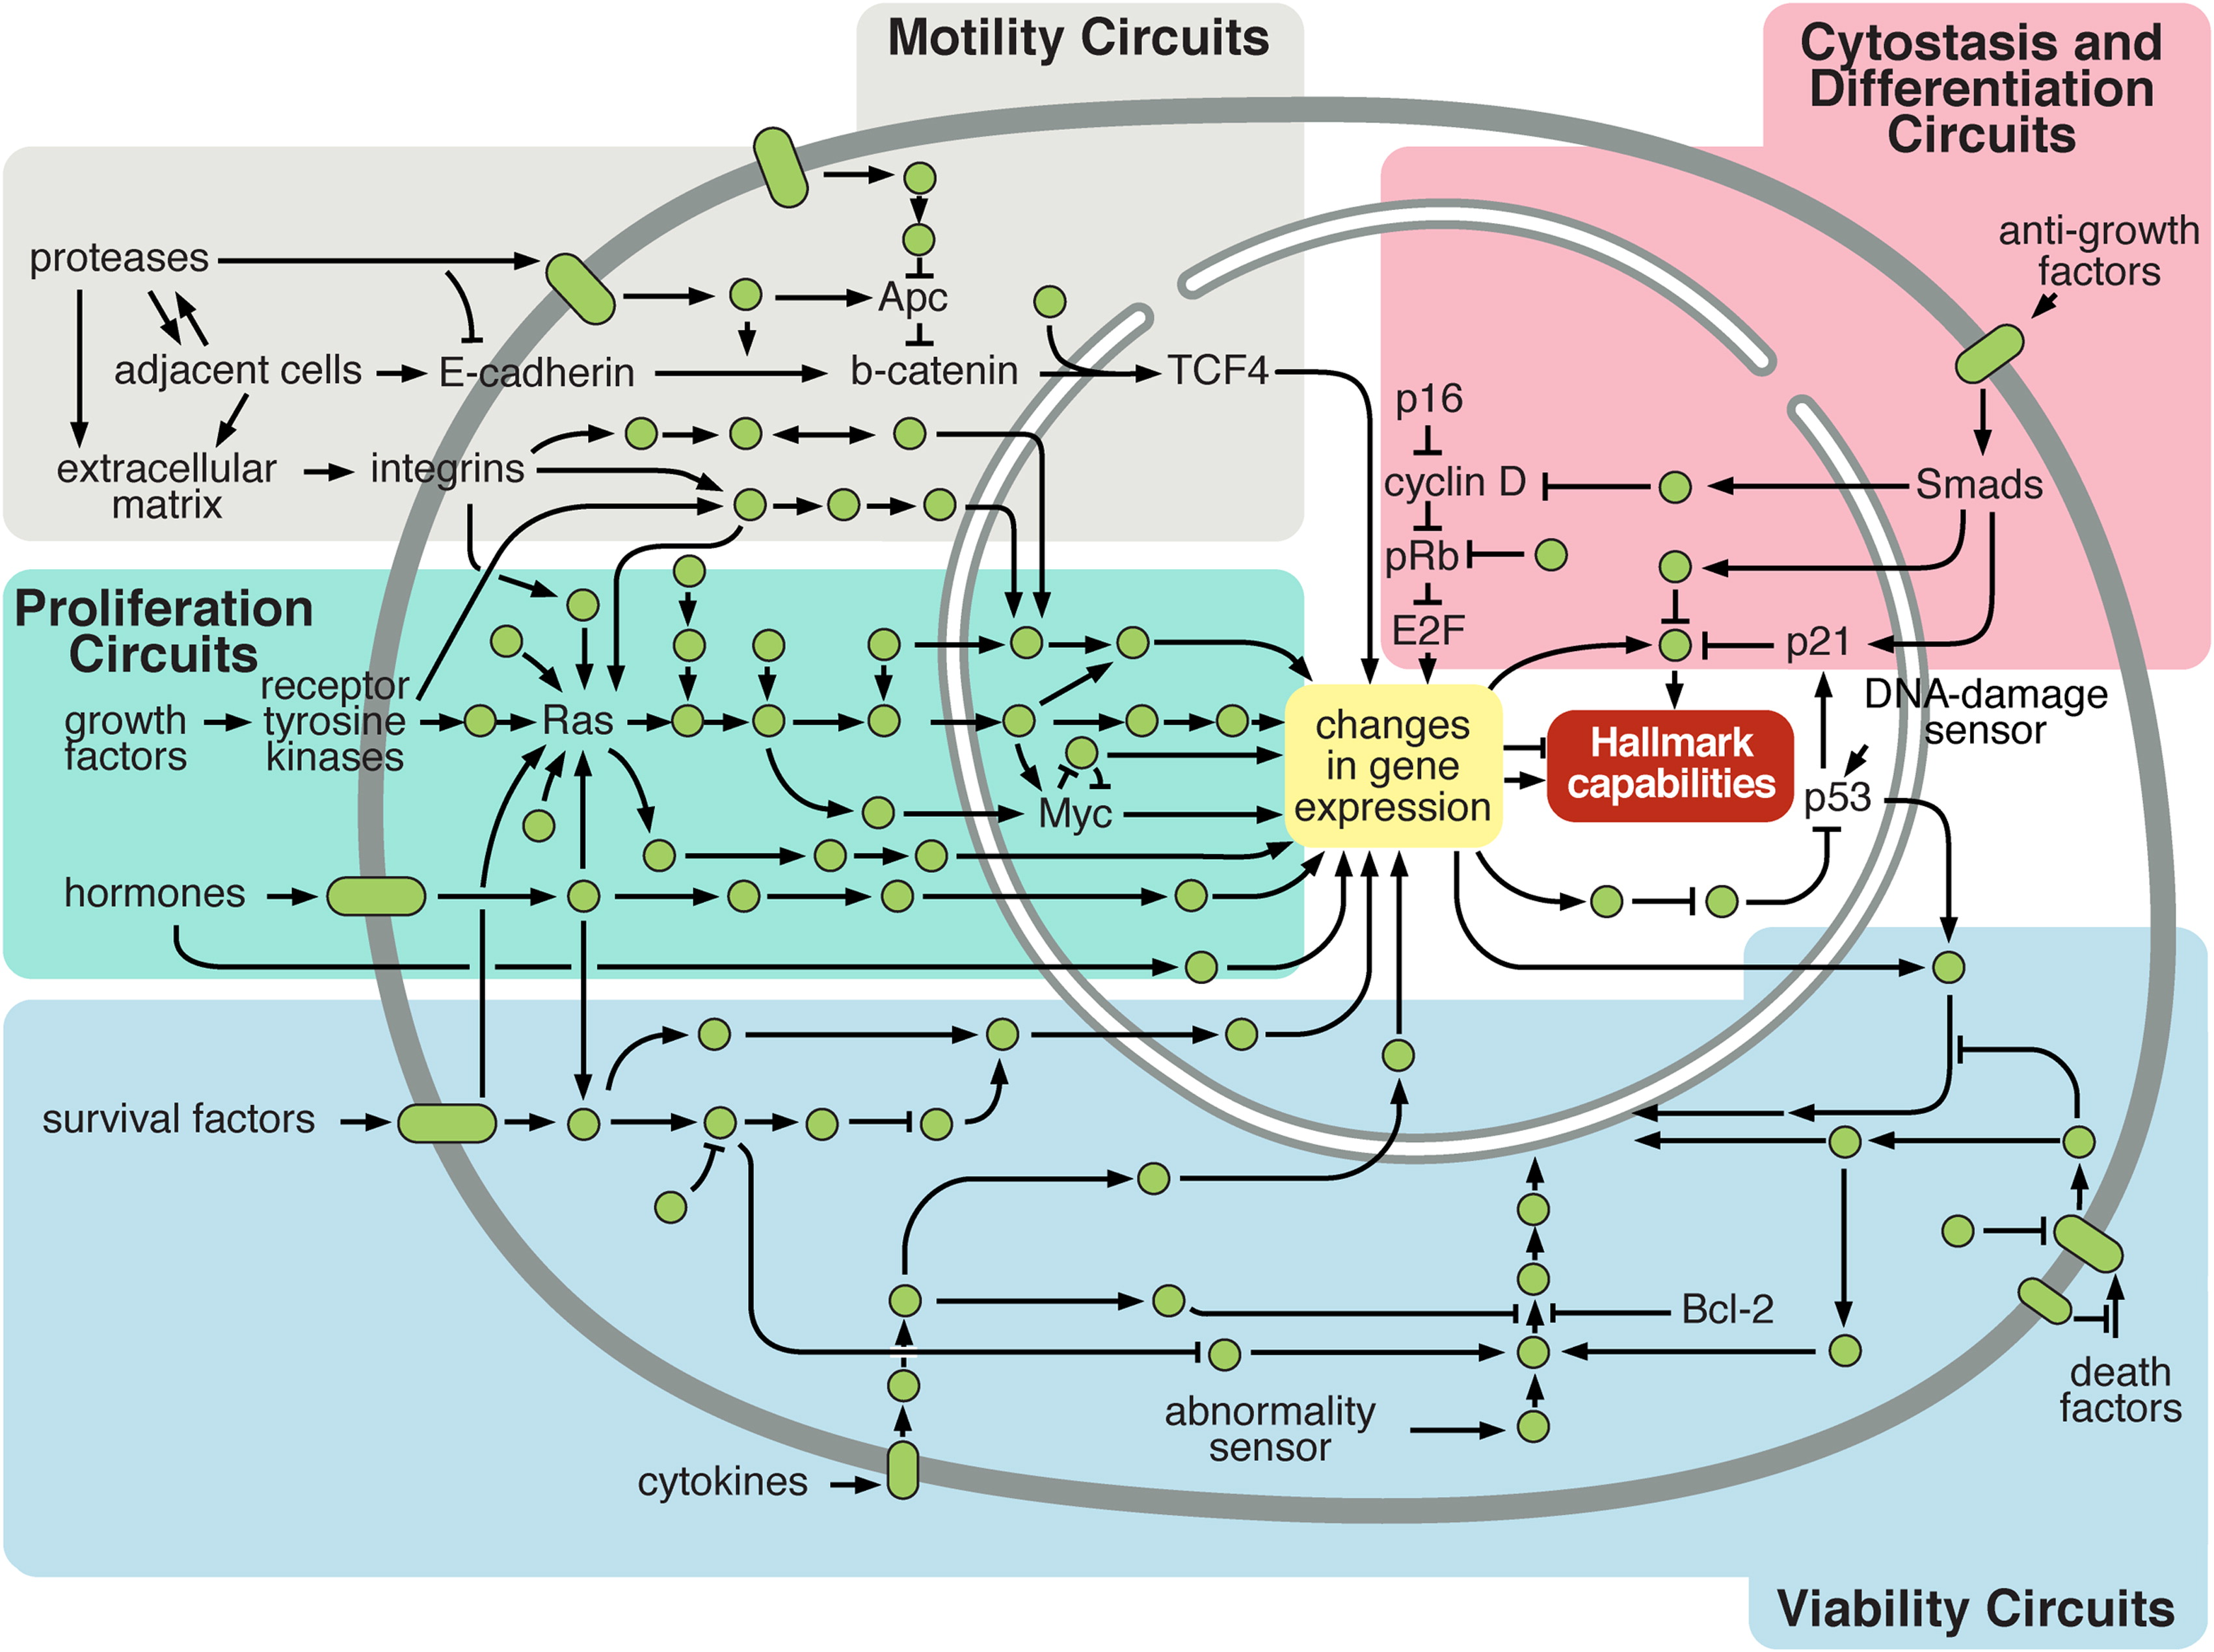
\includegraphics[height=0.9\textheight]{figures/cancer_signalling}
    \end{center}
\end{frame}

\begin{frame}{Complex (or multifactorial) diseases}
    \begin{itemize}
        \item Do \alert{not} have a single genetic cause
        \item Likely associated with the effects of:
              \begin{itemize}
                  \item Multiple genes
                  \item Lifestyle and environmental factors
                  \item Foetal programming?
              \end{itemize}
    \end{itemize}
    \vfill
    Compare with:
    \begin{itemize}
        \item Genetic disorders
        \item Infectious diseases
    \end{itemize}
\end{frame}

\begin{frame}{Biological scale}
    \begin{center}
        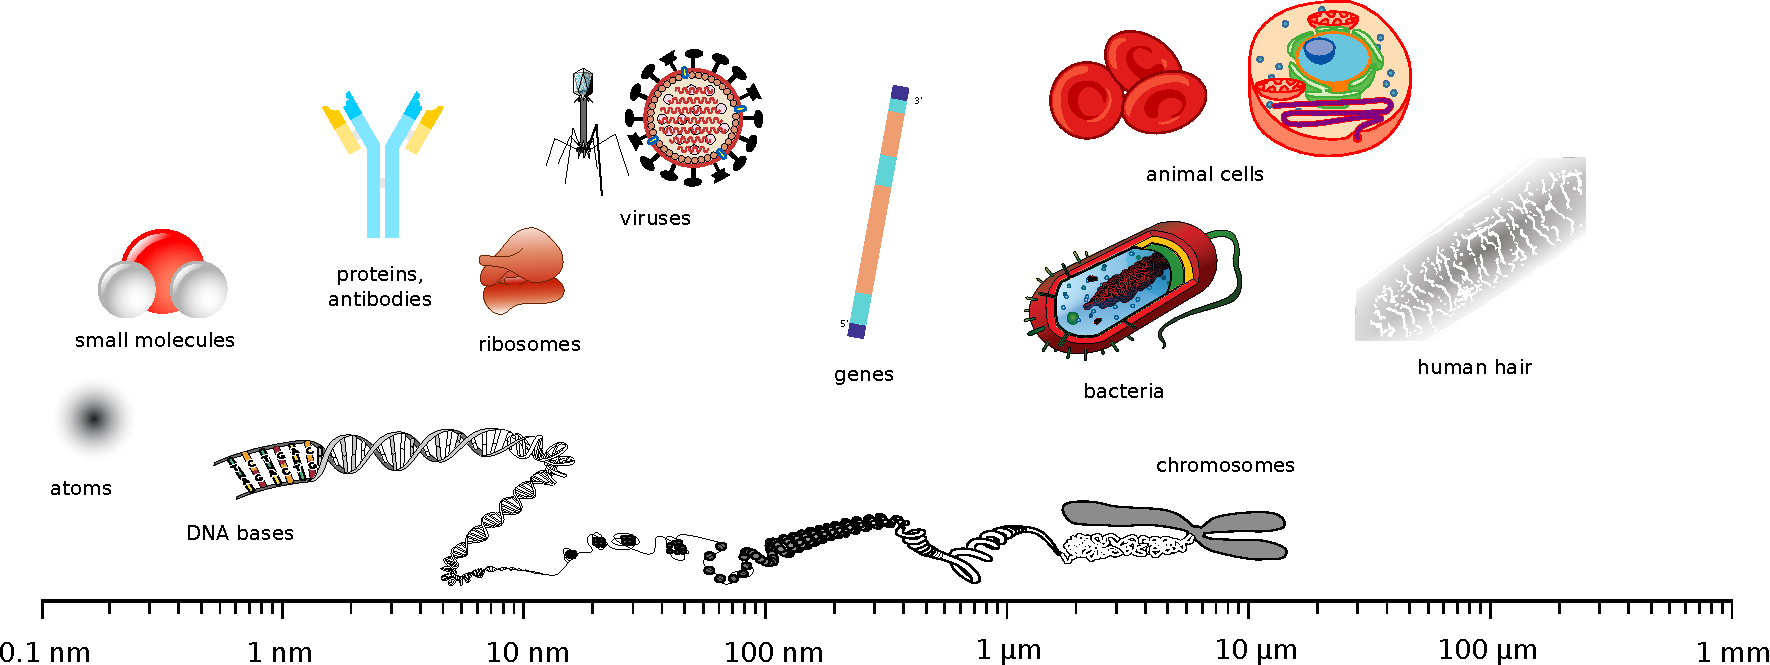
\includegraphics[width=\textwidth]{figures/bio_scale}
    \end{center}
\end{frame}

\begin{frame}{The `central dogma' of molecular biology}
    \begin{center}
        \large%
        \alert{`DNA makes RNA makes proteins'}
    \end{center}
    \vfill
    \begin{block}{General transfers}
        \begin{enumerate}
            \item Replication (DNA $\rightarrow$ DNA)
            \item Transcription (DNA $\rightarrow$ RNA)
            \item Translation (RNA $\rightarrow$ proteins)
        \end{enumerate}
    \end{block}
    \vfill
    \begin{block}{Special transfers}
        \begin{enumerate}
            \item Reverse transcription (RNA $\rightarrow$ DNA)
            \item RNA replication (RNA $\rightarrow$ RNA)
        \end{enumerate}
    \end{block}
\end{frame}

\begin{frame}{Information flow: DNA $\rightarrow$ RNA $\rightarrow$ proteins}
    \begin{center}
        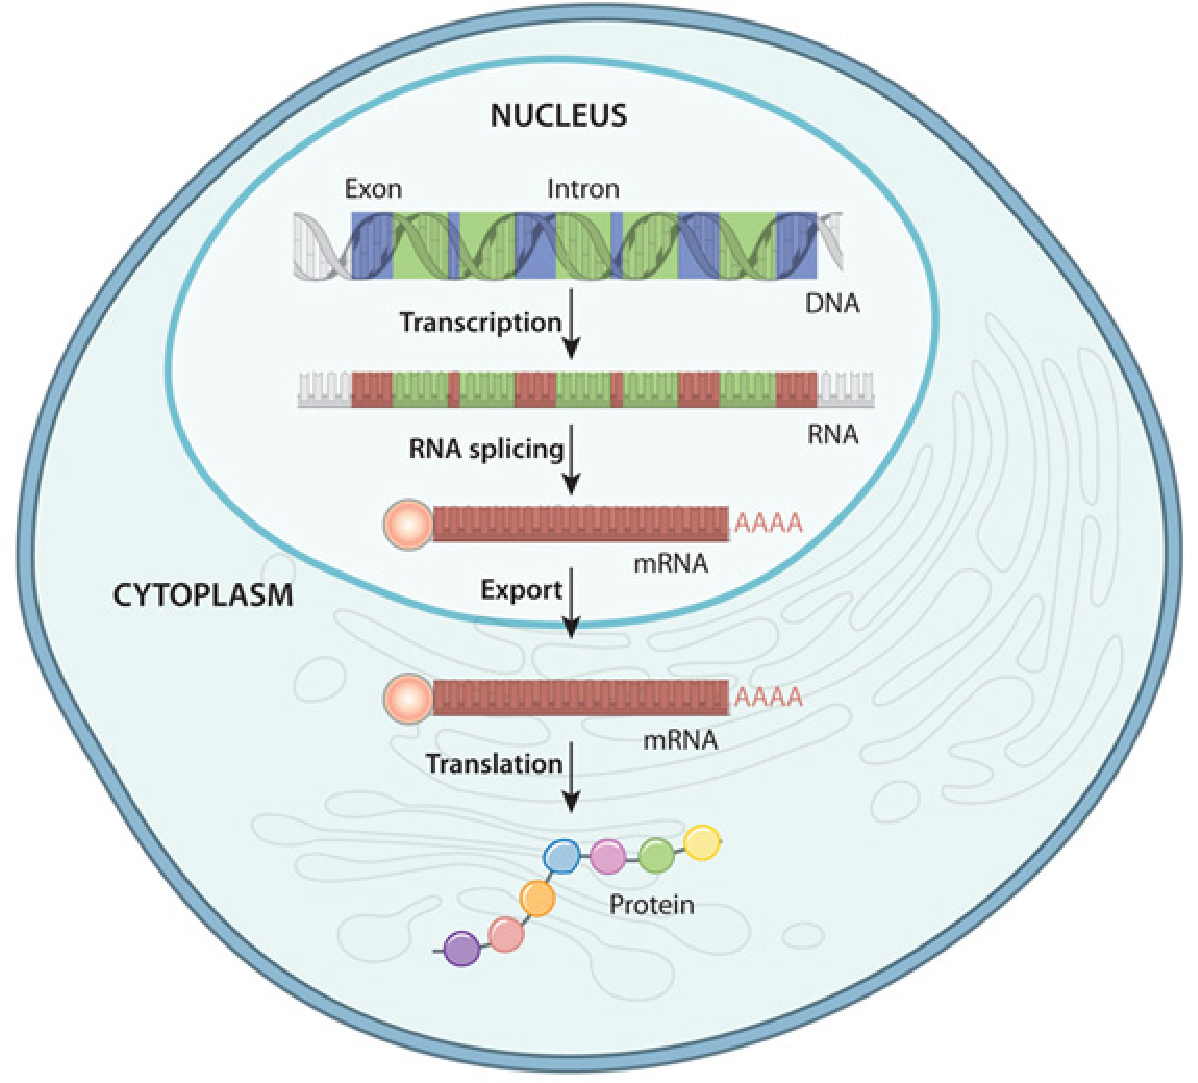
\includegraphics[height=0.9\textheight]{figures/information_flow}
    \end{center}
\end{frame}

\begin{frame}{Regulation of gene expression}
    \begin{block}{Transcriptional regulation}
        \begin{itemize}
            \item \textit{Cis}/\textit{trans} regulation
            \item Epigenetics (DNA methylation and histone modifications)
        \end{itemize}
    \end{block}
    \vfill
    \begin{block}{Post\hyp{}transcriptional regulation}
        \begin{itemize}
            \item Co\hyp{}transcriptional modification
            \item miRNAs
        \end{itemize}
    \end{block}
    \vfill
    \begin{block}{Post\hyp{}translational regulation}
        \begin{itemize}
            \item Modification (reversible)
            \item Degradation (irreversible)
        \end{itemize}
    \end{block}
\end{frame}

\begin{frame}{Epigenetics}
    \begin{block}{DNA methylation}
        \begin{itemize}
            \item Methyl groups (--CH$_{3}$) attached to cytosines
            \item Usually (but not exclusively) at C followed by G
                  (\alert{CpG loci})
            \item Most CpG loci clustered in dense `CpG islands'
            \item Effect on transcription dependent on location
        \end{itemize}
    \end{block}
    \vfill
    \begin{block}{Histone methylation and acetylation}
        \begin{itemize}
            \item Methyl/acetyl groups (--COCH$_{3}$) attached to histone
                  tails
            \item Very complex (combinatorial) effects on transcription
        \end{itemize}
    \end{block}
\end{frame}

\begin{frame}{Why regulate gene expression?}
    \begin{columns}
        \begin{column}{0.5\textwidth}
            \begin{center}
                \large%
                \alert{Differentiation} \\
                into different cell types

                \vspace{2\bigskipamount}

                Response to \\
                \alert{acute and chronic stress}
            \end{center}
        \end{column}
        \begin{column}{0.5\textwidth}
    \begin{center}
        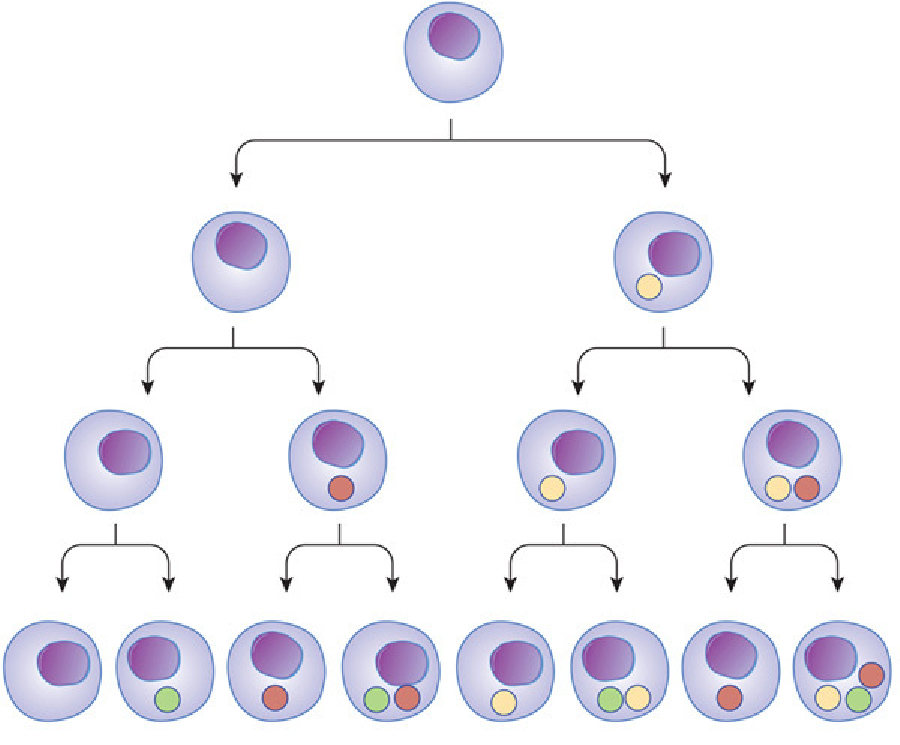
\includegraphics[width=\textwidth]{figures/differentiation}
    \end{center}
        \end{column}
    \end{columns}

\end{frame}

\begin{frame}{Complex diseases: deregulation of information flow?}
    \begin{center}
        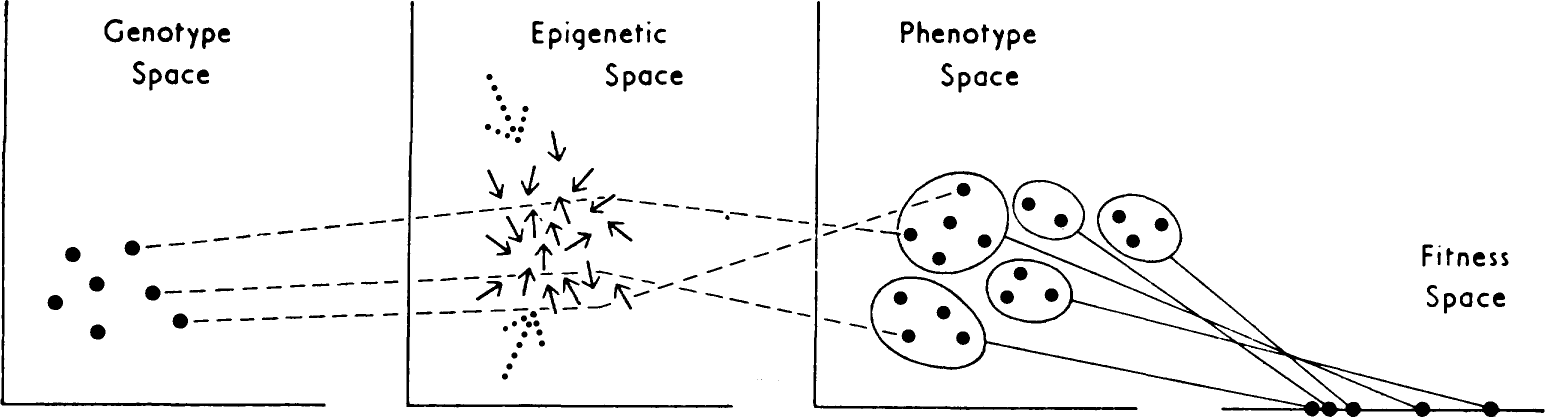
\includegraphics[width=\textwidth]{figures/epi_landscape} \\
        {\scriptsize%
         From Scarr and McCartney (1983)}
    \end{center}
\end{frame}

\begin{frame}{Complex diseases: there is more\ldots}
    \begin{center}
        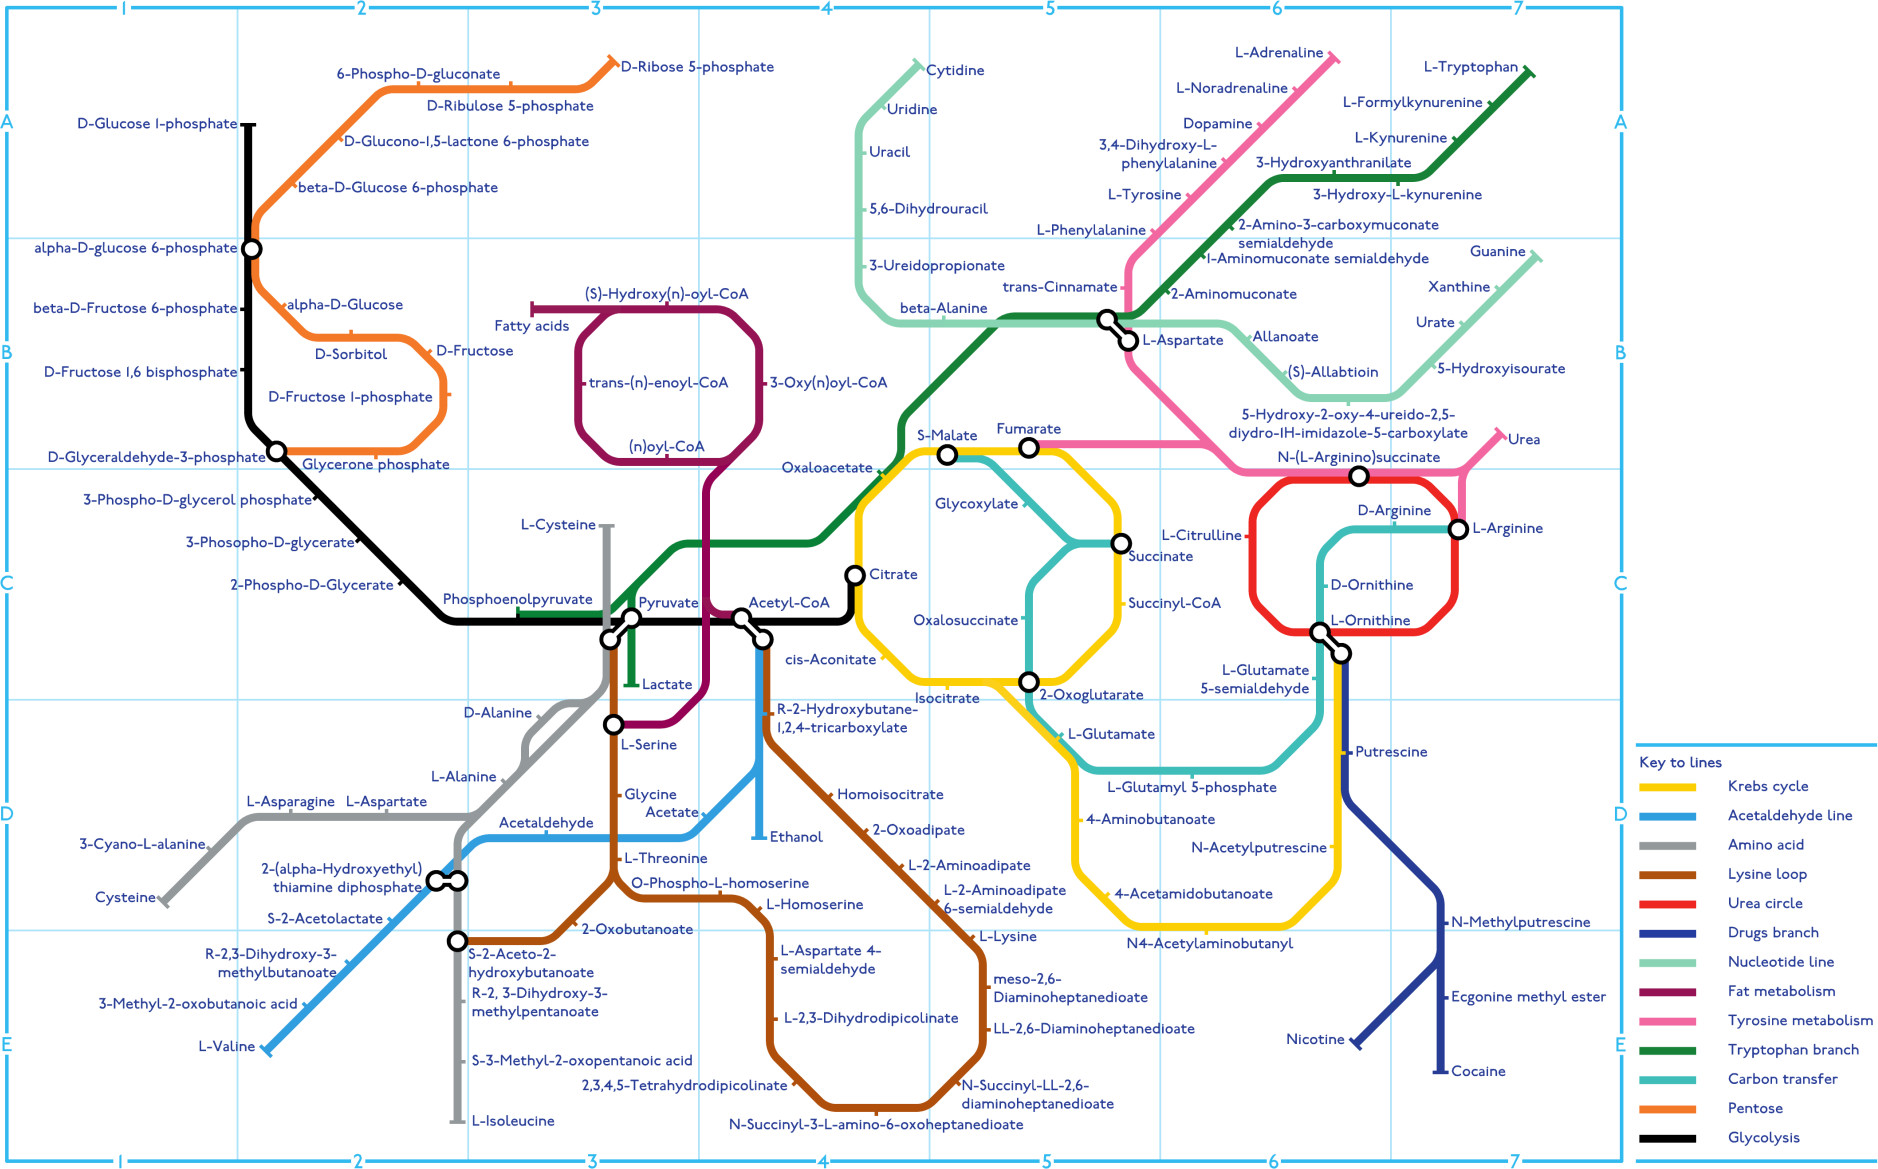
\includegraphics[height=0.9\textheight]{figures/metabolism}
    \end{center}
\end{frame}

\begin{frame}{Of `--omes' and `--omics'\ldots}
    \begin{block}{`--ome'}
        Forming nouns with the sense `all of the specified constituents of a
        cell, considered collectively or in total'
    \end{block}
    \vfill
    \begin{block}{`--omics': the study of `--omes'?}
        \begin{itemize}
            \item \alert{Collective} characterization of the building blocks of
                  structure, function, and dynamics of organisms
            \item \sout{Hypothesis\hyp{}free} Agnostic
        \end{itemize}
    \end{block}
\end{frame}

\section{Technologies}

\begin{frame}{Overview}
    \begin{center}
        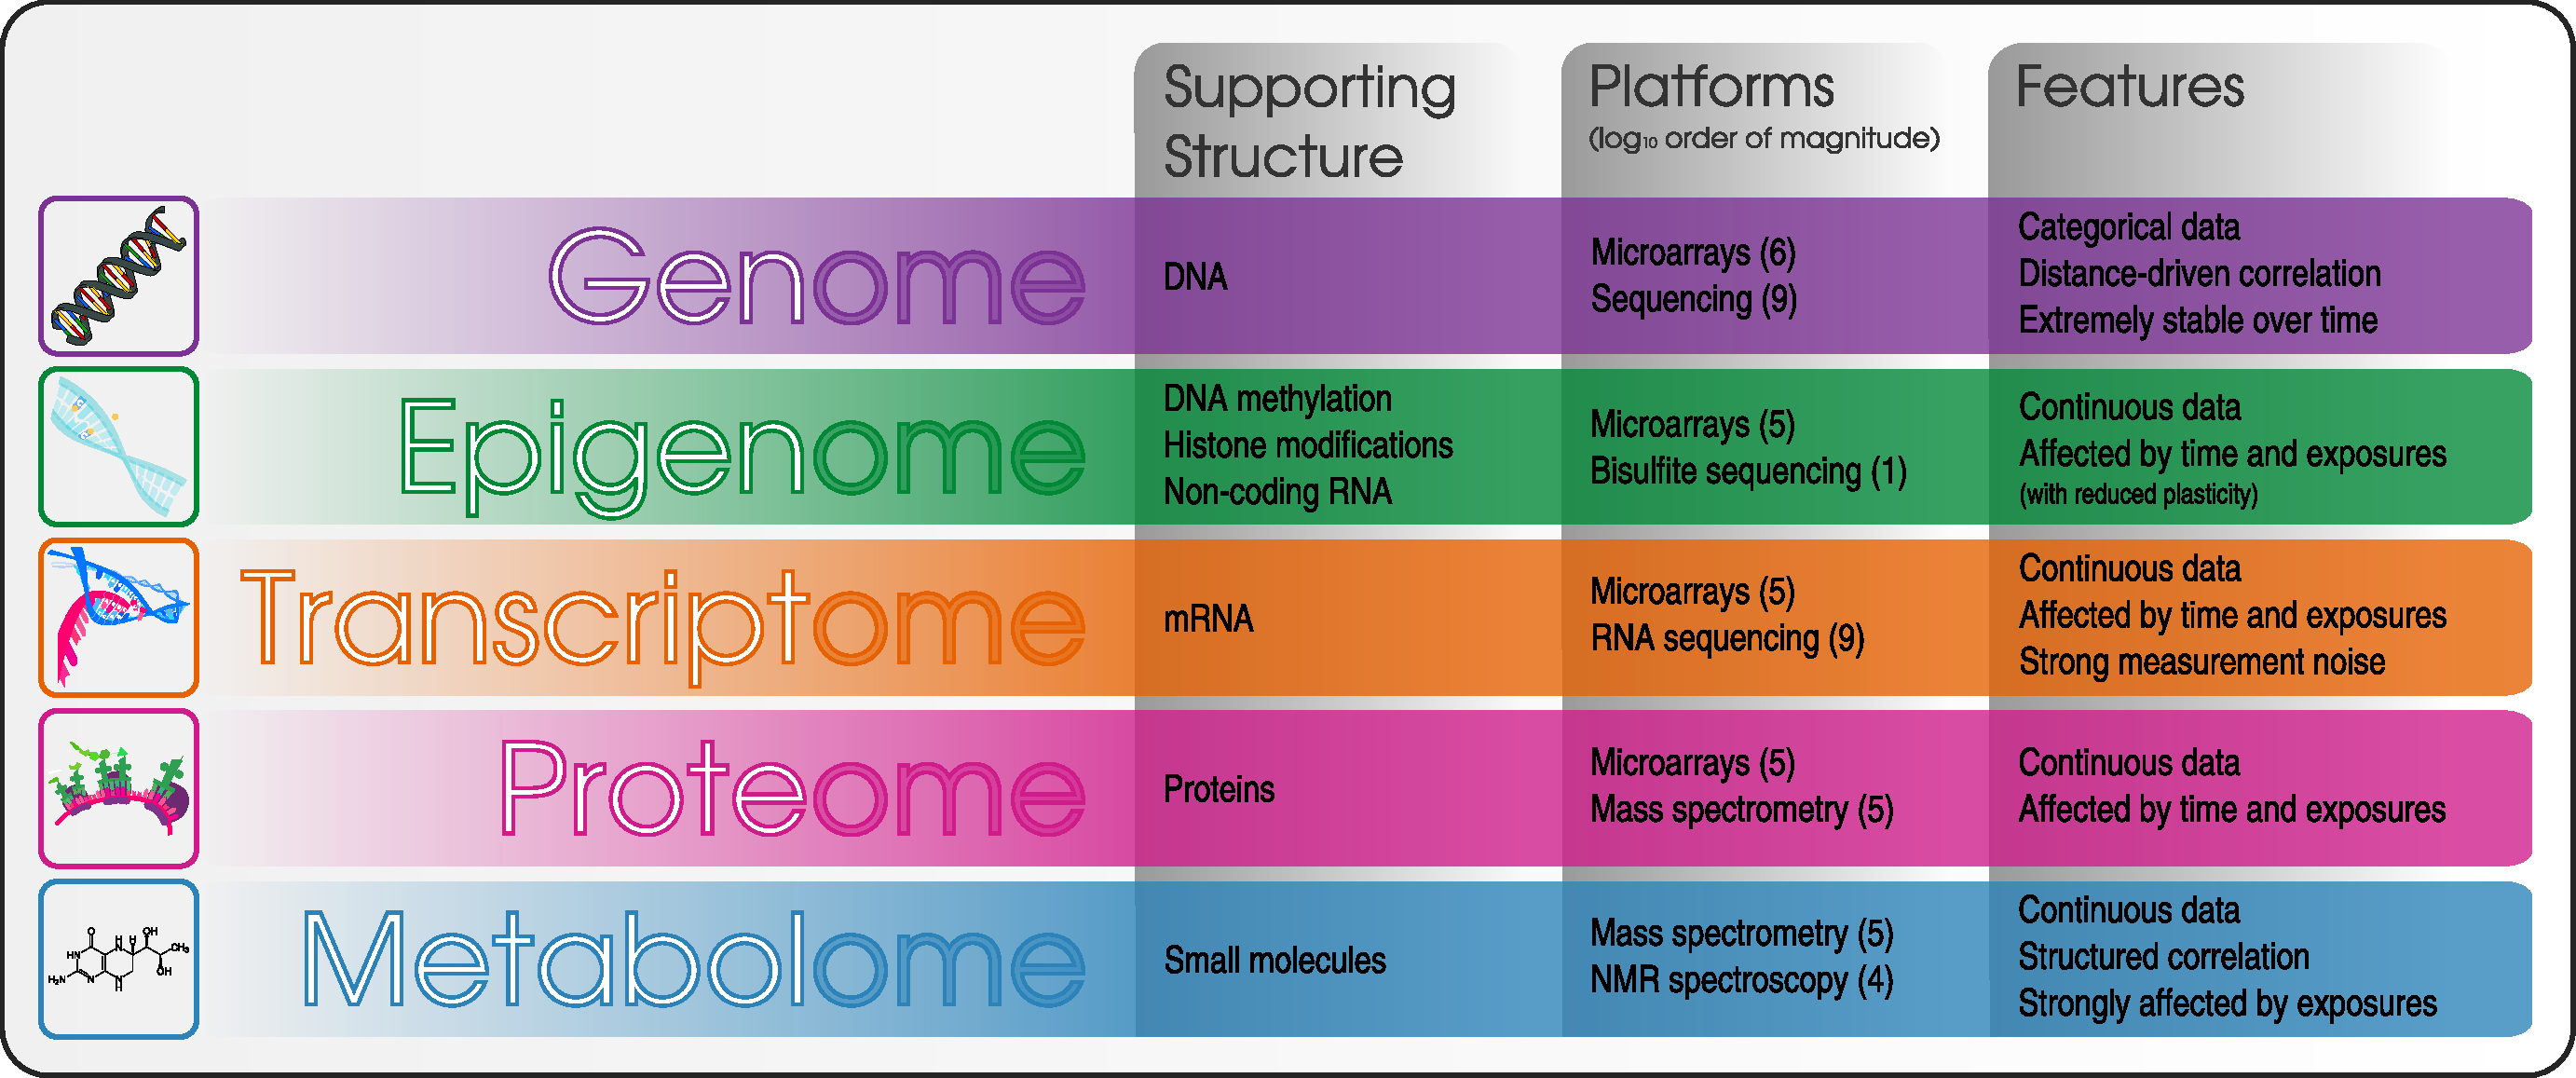
\includegraphics[width=\textwidth]{figures/omics}
    \end{center}
\end{frame}

\begin{frame}{Genomics}
    \only<1>{%
        \begin{block}{Methods}
            \begin{itemize}
                \item Targeted:
                      \begin{itemize}
                          \item Single\hyp{}nucleotide polymorphisms (SNPs)
                          \item Copy\hyp{}number variations (CNVs)
                      \end{itemize}
                \item Partly targeted: exome sequencing
                \item Untargeted: whole genome sequencing
            \end{itemize}
        \end{block}}
    \only<2>{%
        \begin{block}{Outputs}
            \begin{itemize}
                \item Targeted: alleles or copy number \\
                      $\rightarrow$ Statistical analysis is straightforward
                \item Partly targeted and untargeted: sequence reads \\
                      $\rightarrow$ Must map to reference genome
            \end{itemize}
        \end{block}}
\end{frame}

\begin{frame}{Epigenomics: DNA methylation}
    \only<1>{%
        \begin{block}{Method}
            \begin{enumerate}
                \item Create polymorphisms at methylated cytosines using
                      bisulphite conversion
                      (C $\rightarrow$ U/T, me-C $\rightarrow$ C)
                \item Use genomic methods
            \end{enumerate}
        \end{block}}
    \only<2>{%
        \begin{block}{Output}
            \begin{itemize}
                \item Percentage of methylated cytosines at each CpG locus \\
                      $\rightarrow$ Statistical analysis is (more or less)
                                    straightforward
                \item Average over many cells, possibly of different types
                \item Sequence reads must again be mapped to reference genome
                      after \textit{in silico} `bisulphite conversion'
            \end{itemize}
        \end{block}}
\end{frame}

\begin{frame}{Transcriptomics (and miRNAs)}
    \only<1>{%
        \begin{block}{Methods}
            \begin{itemize}
                \item Targeted: micro\hyp{}arrays
                \item Untargeted: RNA sequencing (RNA\hyp{}seq)
            \end{itemize}
        \end{block}}
    \only<2>{%
        \begin{block}{Outputs}
            \begin{itemize}
                \item Targeted: intensities proportional to RNA abundances \\
                      $\rightarrow$ Statistical analysis is straightforward
                \item Untargeted: sequence reads \\
                      $\rightarrow$ Must map to reference transcriptome \\
                      $\rightarrow$ Must take into account splicing
            \end{itemize}
        \end{block}}
\end{frame}

\begin{frame}{Proteomics and metabolomics}
    \only<1>{%
        \begin{block}{Methods}
            \begin{itemize}
                \item Targeted: mass spectrometry assays
                \item Untargeted: mass spectrometry and NMR spectroscopy
            \end{itemize}
        \end{block}}
    \only<2>{%
        \begin{block}{Outputs}
            \begin{itemize}
                \item Targeted: quantified proteins/metabolites
                \item Untargeted: mass and retention times, or spectra
                \item[$\rightarrow$] Statistical analysis is straightforward,
                                     but unknown compounds from untargeted
                                     studies may be
                                     \alert{very difficult to identify}
            \end{itemize}
        \end{block}}
\end{frame}

\section{Lessons learned}

\begin{frame}[t]{Know your biology}
    \begin{center}
        You need some \alert{knowledge of the biological process}\\
        if you are to model it meaningfully
    \end{center}
    \vfill
    \begin{itemize}
        \item Aim to grasp the subject decently: get a good biology textbook if
              needed, and ask questions
        \item Find out which questions are still unanswered: they make great
              hypotheses to test in your dataset
    \end{itemize}
\end{frame}

\begin{frame}[t]{Know your technology}
    \begin{center}
        You need some \alert{knowledge of the measurement procedure}\\
        if you are to model it meaningfully
    \end{center}
    \vfill
    \begin{itemize}
        \item Read the manuals, possibly several times
        \item Understand \alert{what} is being measured, and \alert{how}
        \item Be aware of quirks in the design!
    \end{itemize}
\end{frame}

\begin{frame}[t]{The plague of batch effects}
    \begin{center}
        Protocols are tedious and involve many complex (and often complicated)
        steps that will introduce \alert{nuisance variation}
    \end{center}
    \vfill
    \begin{enumerate}
        \item \alert{Record} as much information as possible
        \item \alert{Identify} influential factors (QC)
        \item \alert{Attenuate} by means of preprocessing
        \item \alert{Model} any residual confounding
    \end{enumerate}
\end{frame}

\begin{frame}[t]{Know your statistics}
    \begin{center}
        You need some \alert{knowledge of statistical modelling} \\
        if you are to write down a model
    \end{center}
    \vfill
    \begin{itemize}
        \item What is your question?
        \item What assumptions can you reasonably make (and verify)?
        \item What type of data do you have at hand?
        \item Explore different options, but be careful when borrowing methods
              from other fields
    \end{itemize}
\end{frame}

\begin{frame}[t]{Trust, but verify}
    \begin{itemize}
        \item Women with Y chromosome
        \item Controls with date of diagnosis
        \item `Matched' pairs with huge age differences
        \item Secondary instead of primary cancer
        \item Technical replicates with different genotype
    \end{itemize}
    \vfill
    \begin{center}
        \alert{Always check}: it takes little time, and saves future headaches
    \end{center}
\end{frame}

\begin{frame}[t]{Know your computer science}
    \begin{center}
        You need some \alert{knowledge of programming}\\
        if you are working with `--omics' data
    \end{center}
    \vfill
    Given the sheer amount of data, we must
    \alert{standardise and automate statistical analysis} as much as possible
\end{frame}

\begin{frame}[t]{Validation and replication}
    \begin{center}
        No matter how stringent your QC and preprocessing, and how accurate your
        models, \alert{false positive results} will still occur
    \end{center}
    \vfill
    \begin{block}{Validation}
        Are results \alert{reliable}?
        Repeat the experiment using the same samples, but a different lab
        technique
    \end{block}
    \begin{block}{Replication}
        Are results \alert{generalisable}?
        Reproduce the findings using different samples, and possibly a different
        lab technique
    \end{block}
\end{frame}

\begin{frame}{Summary}
    \begin{itemize}
        \setlength{\itemsep}{0.5em}
        \item Complex diseases as deregulation of information flow
        \item The `--omics' paradigm: a holistic point of view
        \item Multidisciplinarity:
              \begin{itemize}
                  \item Biological processes
                  \item Measurement procedures
                  \item Statistical modelling
                  \item Computer science
              \end{itemize}
    \end{itemize}
\end{frame}

\begin{frame}{Opportunities}
    \begin{enumerate}
        \setlength{\itemsep}{0.5em}
        \item Identification of novel biomarkers for:
              \begin{itemize}
                  \item Disease risk
                  \item Exposures
                  \item `\alert{Meet\hyp{}in\hyp{}the\hyp{}middle}' approach
              \end{itemize}
        \item Understanding at a molecular level of:
              \begin{itemize}
                  \item Disease states
                  \item Exposures
              \end{itemize}
        \item Characterisation of \alert{dynamic} molecular environment
        \item Development of new treatments
    \end{enumerate}
\end{frame}

\begin{frame}{Biomedical challenges}
    \begin{itemize}
        \item \textbf{Holistic view} \\
              What is the effect of multiple `--omics' markers?
        \item \textbf{Tissue heterogeneity} \\
              What is the value of `--omics' measurements in samples that
              contain multiple, heterogeneous cell types?
        \item \textbf{Surrogate tissues} \\
              What is the value of `--omics' measurements in surrogate tissues,
              e.g.\ in blood, for localised diseases?
        \item \textbf{Effect sizes} \\
              What is the magnitude of clinically significant changes?
    \end{itemize}
\end{frame}

\begin{frame}{Statistical challenges}
    \begin{itemize}
        \item \textbf{Multiple comparisons} \\
              What significance threshold should be used when performing
              millions of tests simultaneously?
        \item \textbf{Nuisance variation} \\
              How can we distinguish between biological and technical variation?
        \item \textbf{Combined effects} \\
              How can we model the combined effect of multiple `--omics'
              markers?
        \item \textbf{`Crossomics'} \\
              How can we analyse multiple `--omics' datasets jointly?
    \end{itemize}
\end{frame}

\end{document}

